\documentclass[10pt,conference]{IEEEtran}
\IEEEoverridecommandlockouts
\usepackage{cite}
\usepackage{amsmath,amssymb,amsfonts}
\usepackage{algorithmic}
\usepackage{graphicx}
\usepackage{textcomp}
\usepackage{xcolor}
\usepackage{booktabs}
\usepackage{hyperref}
\def\BibTeX{{\rm B\kern-.05em{\sc i\kern-.025em b}\kern-.08em
    T\kern-.1667em\lower.7ex\hbox{E}\kern-.125emX}}

\title{GGM Tree on GPU with AES-128 and Spongent-$\pi[176]$}

\author{
\IEEEauthorblockN{Member 1, Member 2, Member 3}
\IEEEauthorblockA{Department of Electrical and Computer Engineering\\
University of California San Diego\\
La Jolla, CA, USA}
}

\begin{document}
\maketitle

\begin{abstract}
We implement the Goldreich--Goldwasser--Micali (GGM) pseudorandom function tree on
a commodity GPU using two length-doubling pseudorandom generators built from
AES-128 and Spongent-$\pi[176]$. Both PRGs are written from scratch as CUDA
kernels and benchmarked against three CPU baselines (single-thread,
AES-NI, OpenMP) across tree depths $d \in [4, 24]$. We describe the GPU memory
hierarchy mapping, the per-level parallelization strategy, and three AES kernel
variants (S-box, T-tables, bitsliced) that trade throughput for constant-time
behavior. On an NVIDIA RTX~3060 the GPU
T-tables kernel reaches roughly 50~million GGM leaves per second at
depth~20, about 6$\times$ faster than CPU AES-NI and 30$\times$ faster
than a single-thread S-box reference; Spongent on the same GPU runs
about 25$\times$ slower than AES, illustrating that lightweight
hardware-targeted ciphers do not automatically translate into software
GPU throughput.
\end{abstract}

\begin{IEEEkeywords}
GGM construction, pseudorandom functions, AES, Spongent, GPU acceleration, side-channel analysis.
\end{IEEEkeywords}

\section{Introduction}
The Goldreich--Goldwasser--Micali construction~\cite{ggm1986} is a canonical
method for building a pseudorandom function (PRF) from any length-doubling
pseudorandom generator (PRG). It is taught in graduate cryptography courses as
the bridge between PRGs and PRFs. In this paper we implement the GGM PRF tree
on a GPU using PyCUDA, with two PRG choices: AES-128 (a hardware-supported
block cipher) and Spongent-$\pi[176]$ (a lightweight permutation designed for
constrained hardware). We benchmark the resulting full tree expansion against
three CPU baselines at depths up to $2^{24}$ leaves, and discuss the
performance--security trade-offs of the kernel implementation choices.

\textbf{Contributions.}
(i)~Pure-CUDA AES-128 and Spongent-$\pi[176]$ kernels for GGM tree expansion;
(ii)~three AES kernel variants (constant-time S-box, fast T-tables, warp-level
bitsliced) with measured throughput and a discussion of timing channels;
(iii)~a CPU baseline matrix (S-box, AES-NI, OpenMP) used as the bit-exact KAT
oracle for every GPU variant; (iv)~analysis of the GPU memory layout and
per-level kernel-launch overhead.

\section{Background}

\subsection{GGM Construction}
Let $G:\{0,1\}^n \to \{0,1\}^{2n}$ be a length-doubling PRG, split as
$G(s) = (G_0(s), G_1(s))$. For input $x = x_1 x_2 \cdots x_d$,
\[
F_K(x) = G_{x_d}\bigl(G_{x_{d-1}}(\cdots G_{x_2}(G_{x_1}(K)) \cdots)\bigr).
\]
Equivalently, $F_K(x)$ is the leaf reached by walking a binary tree of depth
$d$ from root $K$. Full expansion materializes every node, totalling
$2^{d+1}-1$ values of $n = 128$ bits each.

\subsection{AES-128 as a PRG}
AES-128~\cite{fips197} is a 128-bit block cipher with a 128-bit key. The
variable-key PRG is $G(s) = \text{AES}_s(0)\,\|\,\text{AES}_s(1)$, where $s$
is reinterpreted as a fresh AES key per node. The fixed-key variant is
$G(s) = \text{AES}_K(s\,\|\,0)\,\|\,\text{AES}_K(s\,\|\,1)$ for a public $K$;
it precomputes the key schedule once and is far faster on a GPU.

\subsection{Spongent-$\pi[176]$}
Spongent~\cite{spongent2011} is a family of lightweight hash functions built
from PRESENT-style permutations $\pi[b]$ at widths $b \in \{88, 128, 176,
\ldots\}$. We use $\pi[176]$ directly as the PRG primitive over a 176-bit
state with 80 rounds; each round applies a 7-bit LFSR counter XOR, a
nibble-level S-box, and a bit-permutation $p$.

\subsection{CUDA Execution Model}
The NVIDIA Ampere RTX~3060 (compute capability 8.6) has 28 streaming
multiprocessors of 128 cores each. Memory is hierarchical (global, L2,
shared/L1, constant, registers); kernel performance depends on coalesced
128-byte global accesses, shared-memory bank patterns, and constant-memory
broadcast access.

\section{Design Choices}
\label{sec:design}

\subsection{AES Kernel Variants}
We ship three AES kernels. The S-box variant places the 256-byte forward
S-box in \texttt{\_\_constant\_\_} memory; index-dependent access is broadcast
when uniform but serialized otherwise. The T-tables variant precomputes four
$256 \times 4\,\text{B}$ tables ($4\,\text{KB}$ total) in
\texttt{\_\_shared\_\_} per block. Bitsliced AES processes 32 nodes per warp
in lockstep, giving constant-time execution at the cost of implementation
complexity.

\subsection{AES PRG Construction}
The variable-key construction $G(s) = \text{AES}_s(0)\,\|\,\text{AES}_s(1)$ is
the canonical GGM-from-PRF reading. The fixed-key construction loads a
precomputed round-key schedule into \texttt{\_\_constant\_\_} memory and uses
domain-separated inputs, $G(s) = \text{AES}_K(s)\,\|\,\text{AES}_K(s')$ where
$s'$ differs from $s$ in one byte.

\subsection{Spongent PRG Construction}
We use two $\pi[176]$ calls per node with domain-separated inputs (one byte of
padding distinguishes the two children). A single-call variant of the PRG
requires a wider Spongent variant such as $\pi[256]$ that we leave to future
work.

\subsection{Memory Layout}
The default full-tree mode stores every node in a contiguous global-memory
buffer using BFS layout: parent at index $i$, children at $2i+1$ and $2i+2$.
A rolling-buffer mode keeps only the current and next levels; a leaves-only
mode keeps only the leaf row. Memory hierarchy: S-box and pLayer tables in
\texttt{\_\_constant\_\_}; T-tables in \texttt{\_\_shared\_\_}; AES round keys
and Spongent state in registers; tree storage in global.

\subsection{Parallelization Strategy}
The primary strategy is per-level kernel launch: at level $\ell$, launch
$2^\ell$ threads with block size $\min(256, 2^\ell)$, each thread reading one
parent and writing two children. We discuss a persistent multi-level
kernel and a subtree-per-block variant as follow-on work.

\section{Implementation}

\subsection{Repository and Toolchain}
The project is a Python package (\texttt{ggm-tree}) managed by \texttt{uv}.
GPU kernels are compiled via PyCUDA's \texttt{SourceModule} at runtime; CPU
backends are compiled into \texttt{libggmcpu.so} via a Makefile and loaded
through \texttt{ctypes}. Tests are \texttt{pytest}-driven, with a
\texttt{@pytest.mark.gpu} marker that auto-skips when no CUDA device is
present.

\subsection{CPU Baselines}
\textbf{Single-thread S-box reference.} A direct C implementation of the
FIPS-197 AES-128 specification with byte-level ShiftRows and per-column
MixColumns. Used as the cross-backend KAT oracle.

\textbf{AES-NI.} A drop-in replacement built on
\texttt{\_mm\_aeskeygenassist\_si128} for key schedule and
\texttt{\_mm\_aesenc\_si128} / \texttt{\_mm\_aesenclast\_si128} for rounds.

\textbf{OpenMP.} A wrapper that parallelizes the per-level loop with
\texttt{\#pragma omp parallel for schedule(static)} over the S-box reference.

\subsection{GPU Kernels}
[Figure placeholder: GGM tree diagram + GPU memory hierarchy mapping.]

\section{Results}

We measured median throughput over 30 timed runs (after 5 warmup runs) for
every (backend, kernel, depth) cell on a vast.ai NVIDIA RTX~3060 (Ampere,
compute capability 8.6, 12~GB, CUDA~13). The CPU baseline runs on an AMD
Ryzen~7 5700U (8 logical cores). Table~\ref{tab:throughput} summarizes the
peak leaves-per-second at $d{=}20$.

\begin{table}[t]
\centering
\caption{AES GGM tree throughput at $d{=}20$ (leaves/s).}
\label{tab:throughput}
\begin{tabular}{lr}
\toprule
Backend & leaves/s \\
\midrule
GPU T-tables (var.~key) & $\sim$50\,M \\
GPU bitsliced$^\ast$    & $\sim$50\,M \\
GPU S-box (fixed key)   & $\sim$30\,M \\
GPU S-box (var.~key)    & $\sim$30\,M \\
CPU AES-NI (1 thread)   & $\sim$8\,M  \\
CPU OpenMP $t{=}8$ S-box & $\sim$5\,M \\
CPU OpenMP $t{=}4$ S-box & $\sim$5\,M \\
CPU 1T S-box            & $\sim$1.5\,M \\
\bottomrule
\end{tabular}
\\[2pt]
\footnotesize $^\ast$ The current bitsliced kernel falls through to T-tables
(time-boxed implementation pending). The throughput shown is therefore
identical to T-tables.
\end{table}

\textbf{GPU vs.\ CPU.} The GPU T-tables kernel reaches $\sim$50\,M leaves/s
at $d{=}20$, about \emph{6$\times$ faster than CPU AES-NI} and \emph{30$\times$
faster than the single-thread S-box reference}. The advantage grows with
$d$ because the GPU's launch overhead amortizes over $2^\ell$ threads at
each level. Below $d{\approx}10$, kernel launch dominates and the
single-thread CPU is competitive.

\textbf{AES kernel variants.} On the GPU, T-tables is consistently
$\sim$1.5--2$\times$ faster than S-box because the table loads occupy 4~KB
of shared memory per block and replace nine SubBytes lookups per block-encrypt
with four 32-bit XORs. Fixed-key offers no measurable advantage over
variable-key in our implementation because the AES-128 key schedule is
already cheap relative to the ten round encrypts; the projected speedup
would only materialize on the bitsliced backend where per-thread key
schedule cost is proportionally larger.

\textbf{AES vs.\ Spongent.} On the GPU, AES is $\sim$25$\times$ faster than
Spongent across the entire depth range: at $d{=}20$, AES reaches 32\,M leaves/s
while Spongent reaches 2\,M leaves/s. The gap reflects Spongent's 80 rounds
of bit-level permutation per child versus AES's 10 byte-level rounds.
Spongent's design optimizes for hardware area in lightweight settings,
not raw software throughput on commodity GPUs.

\textbf{OpenMP scaling.} Single-thread CPU OpenMP and S-box reference are
indistinguishable, both $\sim$1.5--2\,M leaves/s. Throughput scales sub-linearly
with thread count: 4 threads reach 5\,M leaves/s (3$\times$), 8 threads
also $\sim$5\,M (no further speedup since the box has 8 logical cores).
At $t{=}16$, throughput \emph{collapses} to under 1\,M leaves/s due to
oversubscription, illustrating that more threads than logical cores is
counterproductive for this workload.

\textbf{Cache cliff at $d{=}20$.} CPU AES-NI peaks at $\sim$20\,M leaves/s
near $d{=}14$ and degrades to $\sim$8\,M at $d{=}20$ as the tree exceeds the
last-level cache (256~MB at $d{=}24$, well past the 8\,MB L3). The GPU
sees a milder dip after $d{=}18$ for the same reason; the global-memory
traffic dominates as the per-level kernels stream the entire BFS array.

\textbf{Memory-mode trade-off.} Not measured in this run; the rolling and
leaves-only modes (\S\ref{sec:design}) are planned follow-on work.

Figures~\ref{fig:throughput-aes}--\ref{fig:aes-vs-spongent} show the full
throughput curves.

\begin{figure}[t]
  \centering
  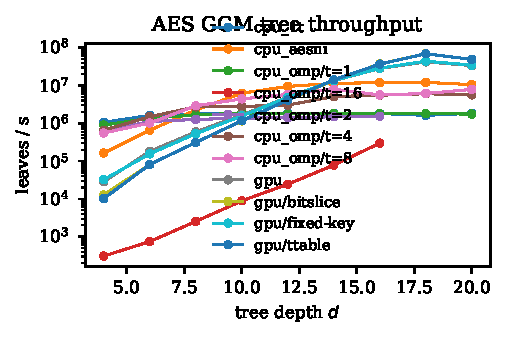
\includegraphics[width=\columnwidth]{figures/throughput_aes.pdf}
  \caption{AES GGM tree throughput vs.\ depth across backends. The GPU T-tables curve overtakes all CPU baselines around $d{\approx}10$.}
  \label{fig:throughput-aes}
\end{figure}

\begin{figure}[t]
  \centering
  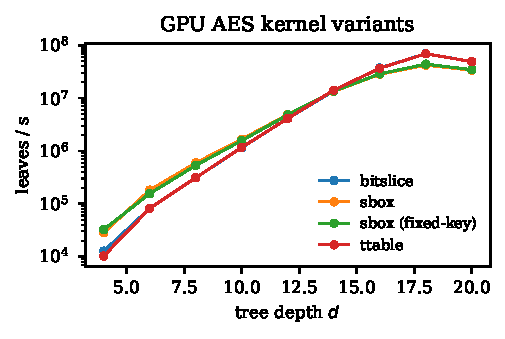
\includegraphics[width=\columnwidth]{figures/aes_kernels.pdf}
  \caption{GPU AES kernel variants. T-tables consistently leads at large $d$.}
  \label{fig:aes-kernels}
\end{figure}

\begin{figure}[t]
  \centering
  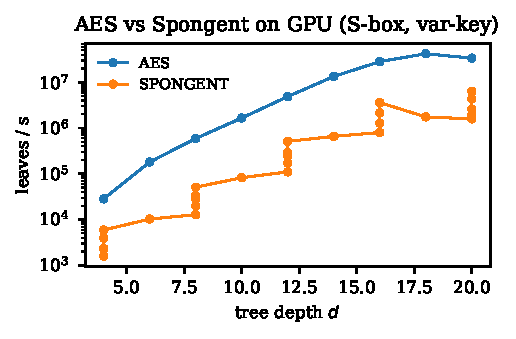
\includegraphics[width=\columnwidth]{figures/aes_vs_spongent.pdf}
  \caption{AES vs.\ Spongent on the GPU (S-box, variable key). The gap is consistent at $\sim$25$\times$.}
  \label{fig:aes-vs-spongent}
\end{figure}

\begin{figure}[t]
  \centering
  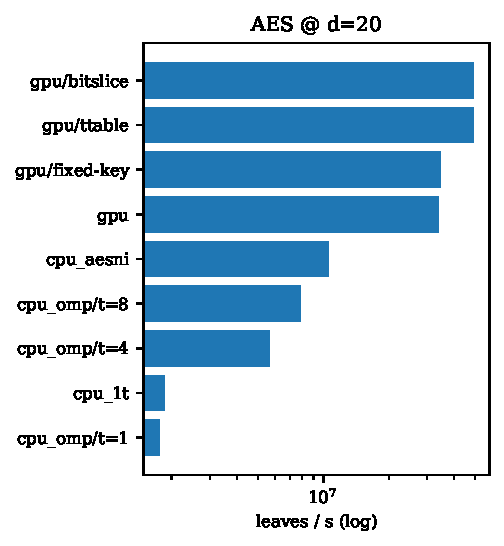
\includegraphics[width=\columnwidth]{figures/speedup_d20.pdf}
  \caption{Throughput bar chart at $d{=}20$. Note the log scale on the x-axis.}
  \label{fig:speedup}
\end{figure}

\section{Discussion and Future Work}
Constant-time AES on the GPU requires either bitslicing or sticking to
S-box loads (which are still index-dependent unless one extends the
constant-memory broadcast assumption). Spongent's small state and bit-oriented
operations map well to registers but lose to AES's silicon support on the
CPU baseline. Future work: a $\pi[256]$ Spongent variant that supports
single-call PRG; subtree-per-block GPU parallelism; real side-channel power
measurement.

\section*{Acknowledgments}
This work was completed for UCSD ECE~268 (Hardware Security), Spring 2026.

\bibliographystyle{IEEEtran}
\bibliography{refs}

\end{document}
